\documentclass[uplatex,dvipdfmx]{jlreq}
\usepackage[fleqn,tbtags]{mathtools}
\usepackage{jlreq-deluxe}
\usepackage[noalphabet]{pxchfon} % must be after otf package
\usepackage{stix2} %欧文＆数式フォント
\usepackage[fleqn,tbtags]{mathtools} % 数式関連 (w/ amsmath)
\usepackage{hira-stix} % ヒラギノフォント＆STIX2 フォント代替定義（Warning回避）
\usepackage{url}

\begin{document}

\title{担当箇所の基本設計・詳細設計のたたき台}
\author{25G1053 齋藤翔太}
\maketitle

\section{システムの基本設計：楽譜データ形式の基本方針}

本システムでは，4種類の楽器パート（主旋律，伴奏など）の楽譜データをPC側ではなく，
各Arduinoノード（node\_02〜05）のメモリ上に保持させる方針とする．

Arduinoの限られたメモリ容量を圧迫しないよう，楽譜データは絶対的な時間（ミリ秒）の配列ではなく，
「音の高さ」と「音の長さ（拍）」のペアからなる相対的なデータとして定義し，
プログラムメモリ上に定数として埋め込む設計とする．
これにより，指揮棒の入力による動的なテンポ変更にも柔軟に対応可能とする．

\section{システムの詳細設計：楽譜データおよび通信仕様}

\subsection{楽譜データの構造設計}

\textbf{1. 課題曲のパート振り分け} \\
課題曲（カエルの歌）を以下の4パートに分割し，各Arduinoへ振り分ける．
\begin{itemize}
    \item node\_02: 主旋律（メロディ）パート
    \item node\_03: 輪唱パート1
    \item node\_04: 輪唱パート2
    \item node\_05: ベース・リズム伴奏パート
\end{itemize}

\textbf{2. データの記述形式} \\
各音符は，以下の2つの要素を組み合わせた構造体（または2次元配列）として定義する．
\begin{itemize}
    \item \textbf{音の高さ (Pitch)}: MIDIノート番号（例: 真ん中のド=60）．休符は0や-1などの特定の数値で定義する．
    \item \textbf{拍・リズム (Duration)}: 四分音符を基準（1.0）とした相対的な音価（例: 八分音符=0.5，二分音符=2.0）．
\end{itemize}

\textbf{3. データ構造の具体例（カエルの歌 冒頭）} \\
主旋律（node\_02）に持たせるデータ配列のイメージを以下に示す．
\begin{table}[ht]
    \centering
    \begin{tabular}{|c|c|c|c|}
        \hline
        順番 & 音階 (Pitch) & 長さ (Duration) & 実際の音 \\ \hline
        1 & 60 & 1.0 & ド（四分音符） \\ \hline
        2 & 62 & 1.0 & レ（四分音符） \\ \hline
        3 & 64 & 1.0 & ミ（四分音符） \\ \hline
        4 & 65 & 1.0 & ファ（四分音符） \\ \hline
        5 & 64 & 1.0 & ミ（四分音符） \\ \hline
        6 & 62 & 1.0 & レ（四分音符） \\ \hline
        7 & 60 & 1.0 & ド（四分音符） \\ \hline
        8 & -1 & 1.0 & （四分休符） \\ \hline
    \end{tabular}
\end{table}

\textbf{4．実装イメージ} \\
定義したデータ形式をArduinoの多次元配列として記述した例を以下に示す．
\begin{verbatim}
int score[][2] = {
  {60, 1.0}, // ド
  {-1, 1.0}, // 四分休符（1拍分，音を鳴らさずに待機）
  {62, 1.0}  // レ
};
\end{verbatim}
このように，音階と音価をセットで管理することで，テンポの変更にも柔軟に対応可能な設計としている．

\subsection{ArduinoからPCへの通信フロー}

各Arduino（node\_02〜05）からPC（Processing）へ送る「音データ」の通信仕様および処理の流れを以下の図に示す．

\begin{figure}[ht]
    \centering
    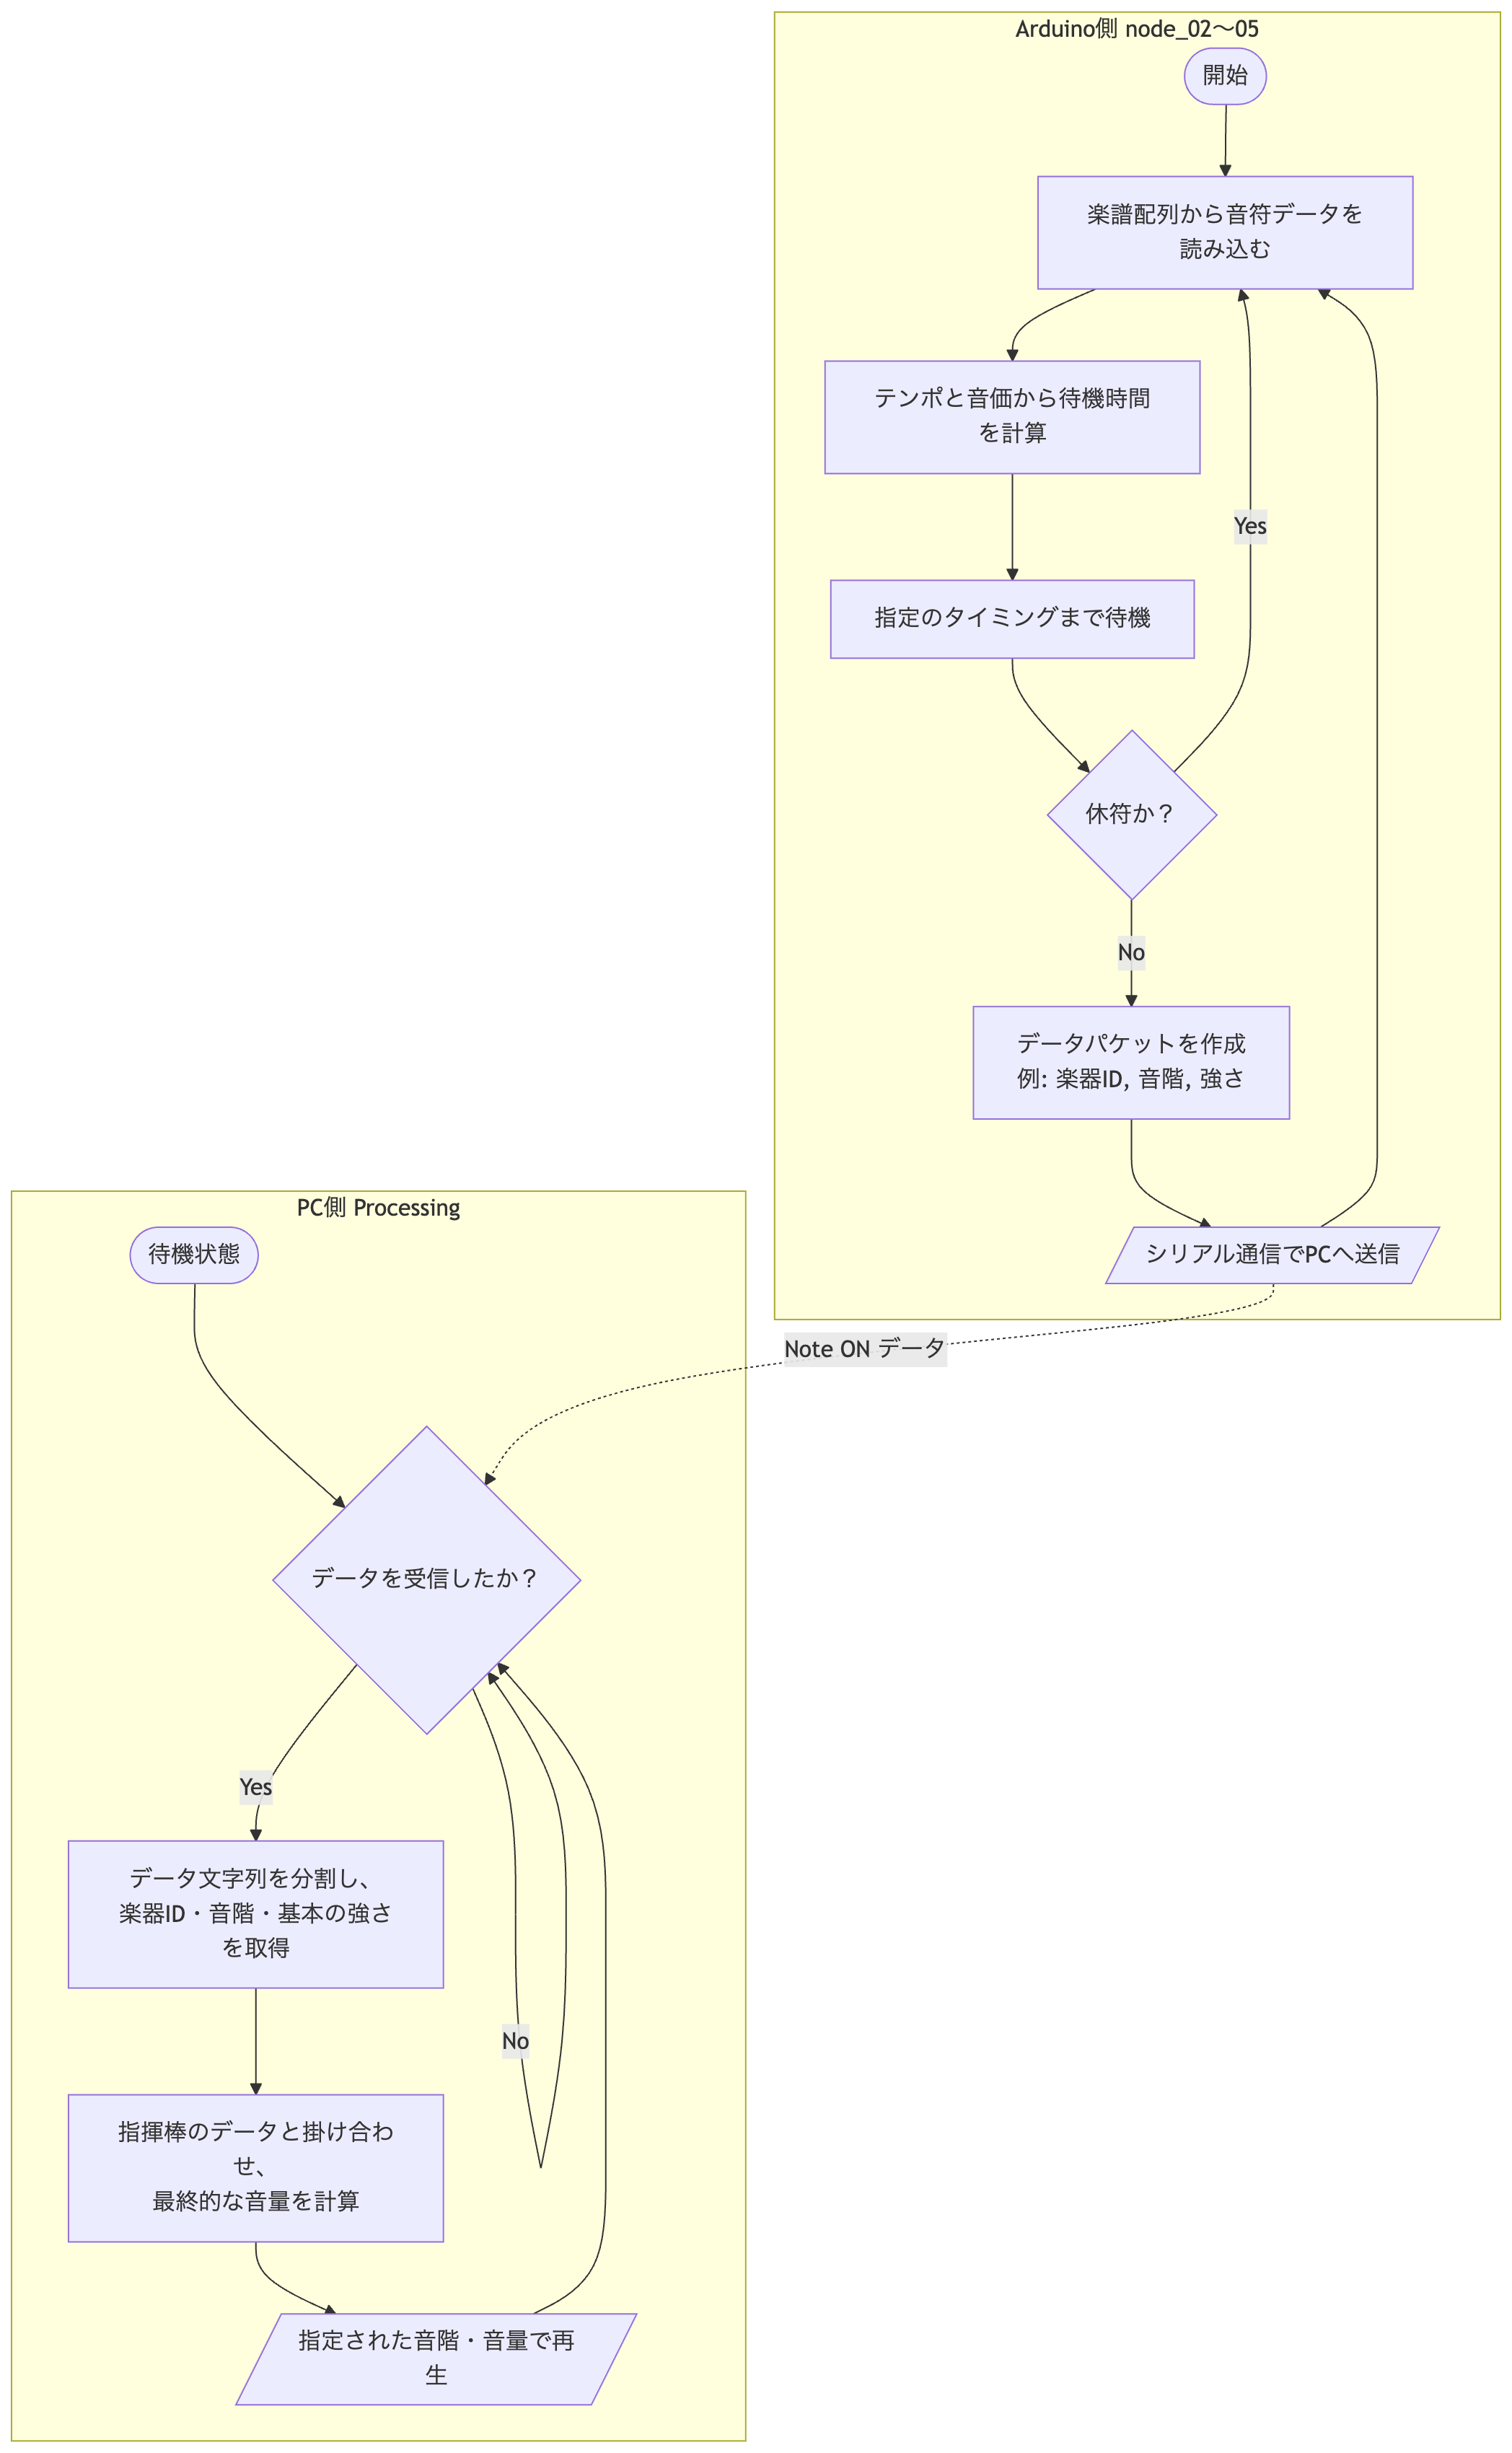
\includegraphics[width=9cm]{flow1.png}
    \caption{ArduinoとPC間の通信および処理フロー}
\end{figure}

\begin{itemize}
    \item \textbf{送るタイミング}: 各Arduinoが自身の持つ楽譜データと現在のテンポを計算し，リアルタイムに送信する．
    \item \textbf{送る内容}: 「どのノードからか（楽器ID）」「どの高さの音か（Pitch）」「音の強さ（Velocity）」の3要素をカンマ区切りなどで送信する．
    \item \textbf{データの粒度}: 音符1つが発音されるごとの「Note ON（発音開始）」単位とする．音の長さ（Duration）の管理は，PC側で行うか，Arduinoから指定時間後に「Note OFF（発音停止）」信号を別途送る仕様とする．
\end{itemize}

\section{生成AIの利用について}
今回作成した基本設計・詳細設計のたたき台は，生成AIのGeminiを利用し，文章の構成や，
誤字脱字のチェックなどに活用した．

\end{document}